\chapter{Materiales}
\section{Parkinson's Progression Markers Initiative (PPMI)} 
\begin{figure}[h]
	\centering
	
\includegraphics[width=0.35\textwidth]{imagenes/ppmi logo.PNG}
	\caption{Logo de la PPMI}
	\label{fig:ppmi}
\end{figure}

La PPMI es un estudio clínico que consiste en el seguimiento de un conjunto de individuos. Su objetivo es facilitar la investigación basada en la búsqueda de identificadores de la progresión de la enfermedad del Parkinson (EP), ya que para poder obtener tratamientos más efectivos es fundamental la detección temprana de marcadores específicos de la enfermedad y comprender su progresión. \cite{HomePark57:online}\\

Este proyecto fue lanzado en el 2010 con la colaboración de investigadores, pacientes y la Michael J. Fox Foundation (MJFF). Entre los pacientes incluidos se encuentran tanto individuos recién diagnosticados de EP, identificados dentro del grupo PD, como sujetos que no la padecen pero que tienen riesgo de de desarrollarla en el futuro, los cuales entran dentro del grupo de control HC, formado por 196 individuos.\\

Dentro del grupo de pacientes que han sido diagnosticados con Parkinson, hay tres subgrupos dentro de los cuales han sido clasificados en función del nivel de desarrollo del declive cognitivo:
\begin{itemize}
	\item PD-CU: Individuos que no presentan deterioro cognitivo. Esta compuesto por un total de 323 pacientes.
	\item PD-MCI: Individuos a los que se les ha detectado un declive cognitivo leve, siendo en total 83 pacientes.
	\item PDD: Individuos diagnosticados con demencia, son un total de 17 sujetos. 
\end{itemize}

Cada uno de los participantes permanece en el estudio durante varios años, permitiendo un seguimiento durante este tiempo en el que se toman medidas de distintos parámetros fundamentales para estudiar la progresión de la enfermedad: marcadores biológicos, evaluaciones clínicas, pruebas de imágenes cerebrales o análisis de líquido cefalorraquídeo. \cite{marek2011parkinson}\\
 
La PPMI permite que la búsqueda de biomarcadores sea más rápida y eficaz, ya que permite la colaboración entre diferentes científicos y el entendimiento de los cambios en el curso clínico entre unos pacientes u otros.


\section{Leaspy}
\begin{figure}[h]
	\centering
	
\includegraphics[width=0.35\textwidth]{imagenes/leaspyLogo.PNG}
	\caption{Logo de Leaspy}
	\label{fig:leaspy}
\end{figure}
Para el análisis de datos con estructura espacial con el objetivo de estimar el
avance de enfermedades, así como para el estudio de datos longitudinales se
desarrollaron las siguientes herramientas de software: Leasp para C++ y Leaspy
para Python. El segundo es utilizado mayoritariamente para estimar la progresión
de enfermedades a largo plazo, imputar valores faltantes y la simulación de
cohortes virtuales.

\subsection{Leasp: Paquete de C++ para el Análisis de Datos Longitudinales
	Estructurados Espacialmente}

Este paquete trabaja con datos obtenidos tras la observación de pacientes a lo
largo del tiempo. Su función se basa en: reconstruir la trayectoria a largo
plazo de los pacientes a partir de las observaciones, ubicar cada medida de cada
paciente en relación con la linea de tiempo promedio grupal y medir el efecto de
ciertos cofactores como por ejemplo el género en el transcurso de la señal. \cite{Welcomet75:online}\\

Esta herramienta puede trabajar tanto con variables escalares, como puntuaciones
clínicas o evaluaciones cognitivas; como con 	datos de red (PET SUVR).\\

El diseño de Leasp se centra en la interacción entre un algoritmo y un modelo
basado en entradas escalares y de red. Con esta biblioteca se tiene acceso a
distintas carpetas que permite el uso de varias funcionalidades:
\begin{itemize}
	\item Aplicación de procedimientos matemáticos
	\begin{itemize}
		\item Calibración
		\item Personalización
		\item Simulación
	\end{itemize}
	\item Funciones de procesamiento
	\item Herramientas de visualización
\end{itemize}

Para su correcta utilización a continuación se muestran algunas instrucciones y
pasos que se deben seguir:

\begin{description}
	\item {\textbf{Requisitos.}} Es necesario instalar las siguientes bibliotecas:
	\textit{tinyxml} (lectura y preprocesamiento de archivos xml),
	\textit{googletest} (pruebas de unidad y funcional ) y  \textit{Armadillo} (uso
	de algebra lineal para vectores y matrices) 
	
	\item {\textbf{Instalación.}} Desde la terminal, ejecutar los comandos que se
	muestran a continuación:
	\begin{enumerate}
		\item \texttt{git clone https://gitlab.com/icm-institute/aramislab/leasp}
		\item \texttt{git submodule init}
		\item \texttt{git submodule update}
		\item \texttt{. mkdir build \&\& cd build}
		\item \texttt{. cmake --options}
		\item \texttt{. make --options\}}
	\end{enumerate}
	
	\item {\textbf{Ejecución del software.}} Agregación del software a
	\texttt{/protect/T1/textdollarPATH} y ejecucion del siguiente comando:
	\begin{center}
		\texttt{leasp fit model\_stgs.xml algorithm\_stgs.xml data\_stgs.xml sampler\_stgs.xml}
	\end{center}
	
	\begin{itemize}
		\item \texttt{fit}: Ajuste de la curva promedia grupal a medidas individuales.
		\item \texttt{model\_settings}: Da información de los parámetros y del tipo de modelo	que se va a ejecutar.
		\item \texttt{algorithm\_settings.xml}: Define parámetros del algoritmo como el numero total de iteraciones.
		\item \texttt{data\_settings.xml}: Recopila la ruta de los archivos de datos.
		\item \texttt{sampler\_settings.xml}: Enumera las muestras utilizadas en el procedimiento de estimación, junto con sus parámetros.
	\end{itemize}
	
	\item {\textbf{Salidas de la estimación.}} Se producen tres archivos en el proceso: \\
	\texttt{convergence\_parameters.csv} muestra la convergencia del modelo.\\ \texttt{population\_parameters.csv} define parametros para el promedio grupal a largo plazo.\\ \texttt{individual\_parameters.csv} que son parametros temporales y espaciales para la trayectoria individual.
\end{description}

\subsection{Leaspy: Toolbox de Python para Aprender Patrones Espaciotemporales de la Progresión de la Enfermedad}

Para el estudio de datos longitudinales y ver la progresión de enfermedades a largo plazo en Python se desarrollo la herramienta Leaspy. Basándose en el modelo de efectos mixtos, permite la reconstrucción de la evolución promedia e individual. Además, permite abordar problemas de los estudios de datos longitudinales, como el que cada paciente tenga un numero de observaciones distinto, permite trabajar con valores faltantes y medidas de datos estructurados espacialmente (imágenes o redes), gracias a la geometría de Riemann. También es de gran utilidad trabajando con medidas en un periodo de tiempo corto, cuando el fenómeno de estudio es de larga duración. Otras aplicaciones permiten predecir puntos temporales futuros y simular nuevas cohortes a partir de los parámetros obtenidos de un ya existente. La calidad del paquete se garantiza mediante pruebas unitarias, control de versiones git e integración continua.
\begin{figure}[h]
	\centering
	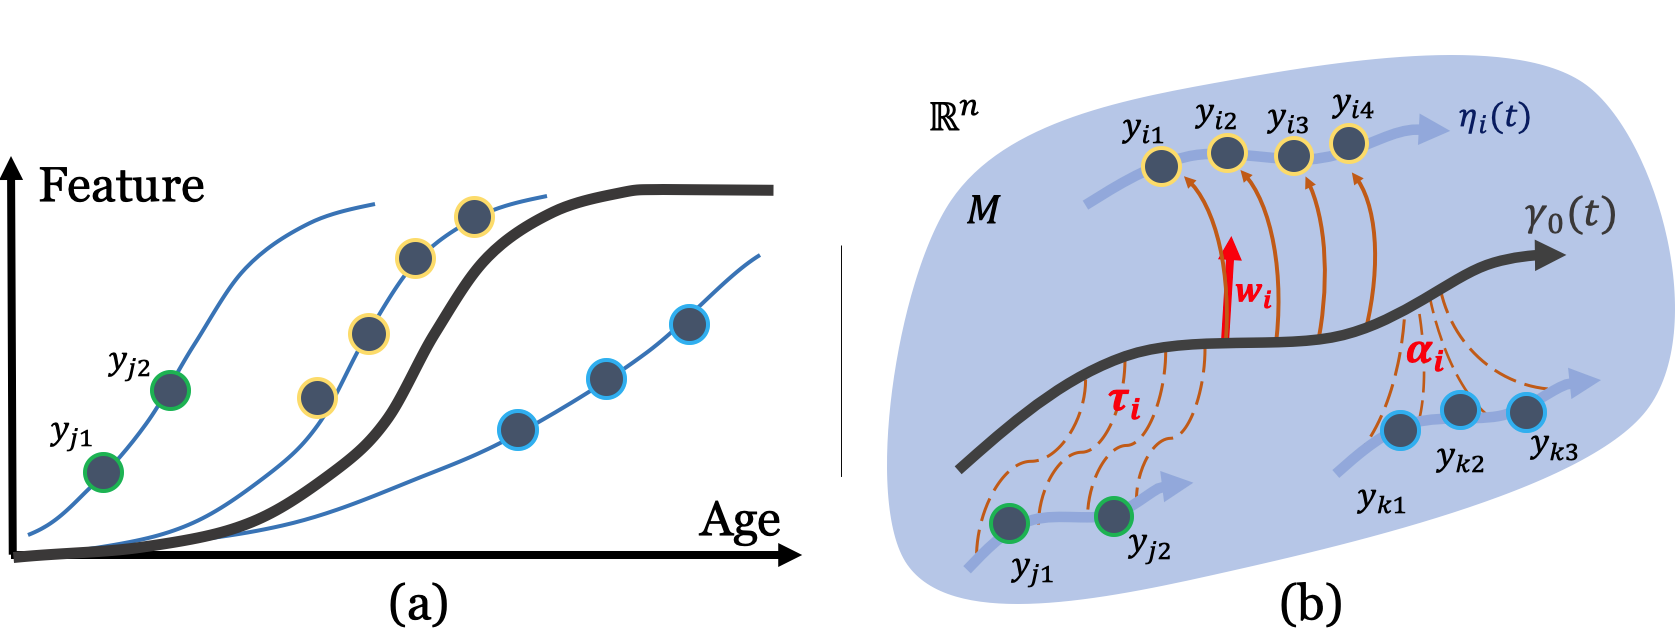
\includegraphics[width=0.9\textwidth]{imagenes/leaspy_trayectories.PNG}
	\caption{Curvas características de la progresión de los marcadores.}
	\label{fig:trayectories}
\end{figure}

El siguiente modelo, basado en efectos mixtos, representa un conjunto de datos longitudinales $y=(y_{ij},t_{ij})\ 1 \leq i \le n, 1 \le j \le k_{i}$ de $\textit{n}$ pacientes. El número de observaciones de cada individuo $i$ se representa con $k_{i}$, siendo los tiempos de cada observación $t_{i1} < ... < t_{ik_{i}}$.

\begin{center}
	$y_{ij} = f(\theta_{geom}, z_{i}, t_{ij} ) + \epsilon_{ij}$
\end{center}

$\theta_{geom}$ son los parámetros del modelo, $z_{i}$ es la variación de cada individuo respecto a la trayectoria promedio grupal y $\epsilon_{ij}$ es un ruido gaussiano. El objetivo es calcular los parámetros anteriores que hagan que los datos sean lo más verosímiles posibles. Con Leaspy se pueden realizar los siguientes procedimientos:
\begin{enumerate}
	\item Calibración: consiste en estimar $y$ a partir de $\theta$, obteniendo la curva promedio del grupo a largo plazo. Esta basada en el algoritmo MCMC-SAEM y la varianza adaptativa y el descenso de gradiente mejoran la velocidad de convergencia.
	\item Personalización: Teniendo $\hat{\theta}$, se reconstruyen las trayectorias individuales obteniendo la variable oculta $z_{i}^{*}$. Este procedimiento estadístico incluye métodos Powell y L-BFGS.
	\item Reconstrucción, imputación de valores faltantes y predicción: Con las variables resultantes de los dos pasos anteriores, se calcula $y_{ij}^{*}=f(\hat{\theta}, z_{i}^{*}, t_{ij})$ para distintos periodos de tiempo.
	\item Simulación: Se genera un individuo completamente nuevo ($z_{i}^{0}$) a partir de $\hat{\theta}$ y un conjunto de variables individuales, pudiendo repetir el proceso hasta conseguir una cohorte virtual. Este método está basado en estimaciones condicionales gaussianas multivariadas y en funciones de densidad kernel.	
\end{enumerate}

La programación en Python de los cuatro procesos anteriores sigue una metodología bastante amigable para le usuario, ya que menos para la reconstrucción, el resto se estructuran de la siguiente manera:
\begin{itemize}
	\item \textbf{Definición de parámetros:} el objeto \texttt{AlgorithmSettings} se encarga de esta función. En su llamada se fija el algoritmo que se quiere utilizar y otras variables. También se pueden cargar a través de kwargs o archivos json.
	\item \textbf{Llamada a las funciones:} tras el paso anterior, se realiza la llamada al método que se este llevando a cabo, introduciendo los parámetros definidos: \texttt{leaspy.fit(...)} para la calibración, \texttt{leaspy.personalize(...)} para personalizar el modelo, \texttt{leaspy.reconstruct(...)} para reconstruirlo y\\\texttt{leaspy.simulate(...)} para realizar una simulación.
	\item \textbf{Visualización y registro:} Leaspy también permite guardar archivos de registro y otras variables en archivos csv y json, lo que también permite volver a cargarlos en el programa; y se pueden visualizar perfiles de progresión o reconstrucciones de trayectorias.
\end{itemize}

Además, para comprender el funcionamiento de este entorno, hay que tener claros los parámetros con los que trabaja Leaspy a la hora de obtener los modelos. \cite{DiseaseC47:online}Por una parte, a la hora de estimar la trayectoria de la progresión media de un biomarcador se utilizan los parámetros \textit{'long-term'}:
\begin{itemize}
	\item $\mathbf{t_{k}}$: Edad para la cual se obtienen los parámetros  que definen la curva general (p0 y u0).
	\item $\mathbf{p_{k}}$: Indica el valor normalizado de la variable en el tiempo t0 para la trayectoria a largo plazo.
	\begin{center}
		$p_{k}=\gamma_{k}(t_{k})$
	\end{center}
	\item $\mathbf{u_{k}}$: Representa la velocidad de aumento del valor de dicha variable en función del tiempo.
	\begin{center}
		$u_{k}=\frac{d}{dt}(\gamma_{k}(t_{k}))$
	\end{center}
\end{itemize}
Estás variables permiten estimar la trayectoria global media de cada biomarcador ($\gamma_{k}$). Esto se realiza con la función \textbf{leaspy.fit}, la cual toma las medidas longitudinales de los sujetos de la base de datos y obtiene los parámetros que definen la curva \textit{'long-term'}. Una vez obtemidos los parámetros, la curva se obtiene con la siguiente ecuación:
\begin{center}
	$\gamma_{k}=\frac{1}{1+((\frac{1}{p_{k}}-1)*exp(-\frac{u_{k}*(t-t_{0})}{p_{k}*(1-p_{k})}))}$
\end{center}
\begin{figure}[h]
	\centering
	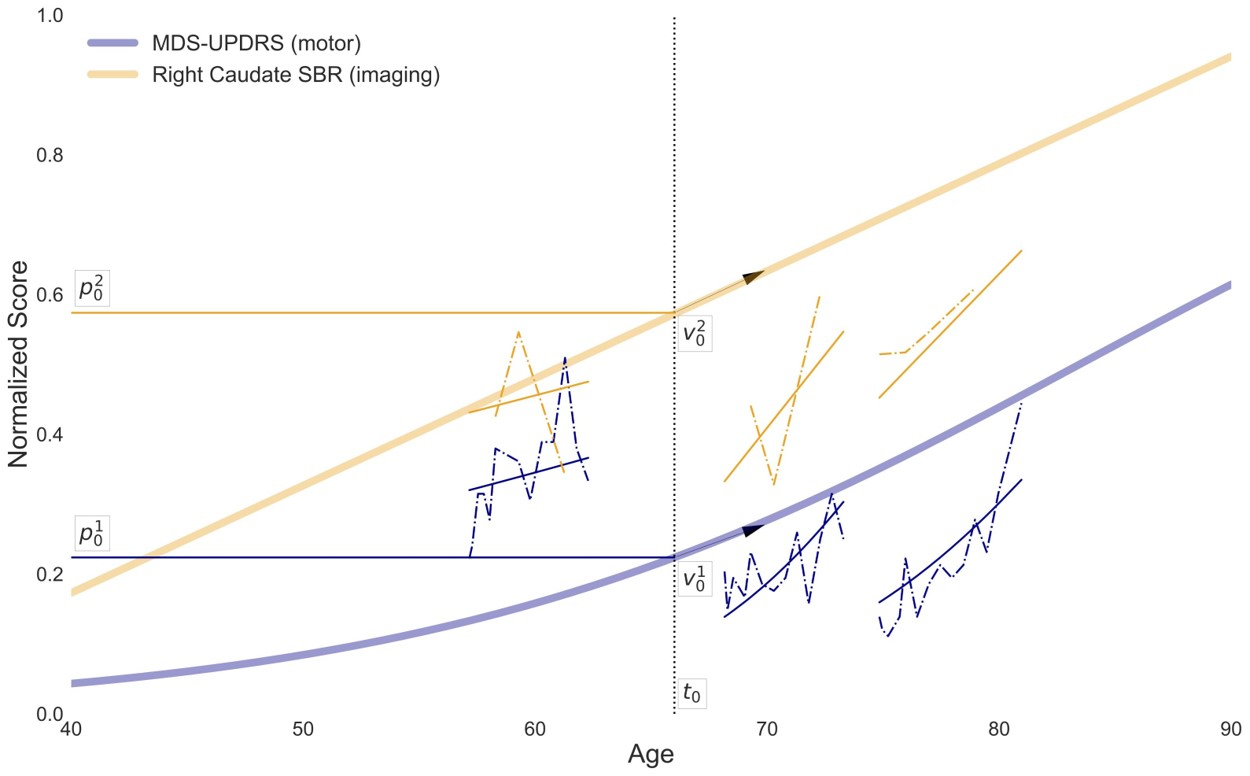
\includegraphics[width=0.85\textwidth]{imagenes/PARÁMETROS LONG TERM.JPG}
	\caption{Representación de los parámetros de una trayectoria long-term}
	\label{fig:long-term}
\end{figure}

Una vez conseguido esto, Leaspy utiliza la función \textbf{leaspy.personalize} para obtener los parámetros \textit{'short-term'}:
\begin{itemize}
	\item $\mathbf{\tau_{i}}$: Representa la reserva cognitiva en años, es decir, el tiempo del que dispone un sujeto antes de alcanzar el declive cognitivo. un valor mayor que 0 indica que la progresión de la enfermedad es más tardía que la media, en cambio un valor negativo indica que que es más temprana.
	\item $\mathbf{\alpha_{i}}$: EL factor de aceleración marca si en el caso del sujeto seleccionado, la enfermedad avanza a mayor velocidad que la media ($\alpha_{i}>1$) o a menos velocidad ($\alpha_{i}<1$).
	\item $\mathbf{w_{ik}}$: El espacio entre marcadores intermedios  indica la secuencia de eventos descrita por el vector $\tau$, que desplaza cada curva logística, propia del paciente.
\end{itemize}
Estas variables representan la curva característica para un nuevo individuo a partir de la trayectoria general obtenida de un grupo de pacientes facilitado. Esta curva se obtiene con la siguiente ecuación en función de los parámetros \textit{'short-term'}:
\begin{center}
	$\eta_k = \frac{1}{1 + \left( \left( \frac{1}{pk} - 1 \right) \cdot e^{-\frac{(w_{ik} + (u_k \cdot \alpha_i \cdot (t_{ij} - t_0 - \tau_i)))}{pk \cdot (1 - pk)}} \right)}
	$
\end{center}
\begin{figure}[h]
	\centering
	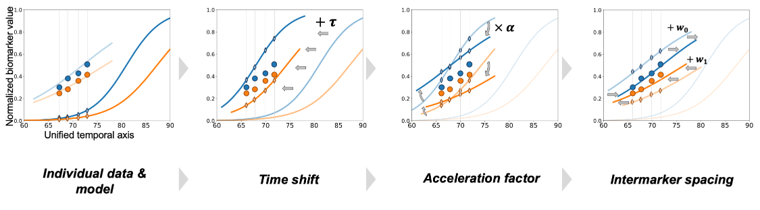
\includegraphics[width=1\textwidth]{imagenes/PARAMETROS SHORT TERM.PNG}
	\caption{Parámetros short-term para la obtención de la curva caracteristica de un nuevo sujeto.}
	\label{fig:short-term}
\end{figure}
Con todas estas herramientas, Leaspy es un entorno versátil y de fácil acceso que permite introducirse en el mundo del análisis y la interpretación de datos longitudinales a través de Python. Permite abordar tareas estadísticas gracias a los modelos y algoritmos en los que esta basado , pudiendo estimara parámetros y simular datos. Además es accesibles desde distintos sistemas operativos como Windows o Linux.

\section{PuTTY}
Está pendiente de introducir ya que todavía no se ha empezado a trabajar con esta herramienta.

\section{Xming}
Está pendiente de introducir ya que todavía no se ha empezado a trabajar con esta herramienta.
